\documentclass{beamer}

\usepackage[french]{babel}
\usepackage[T1]{fontenc}    % Encodage des accents
\usepackage[utf8]{inputenc} % Lui aussi

\mode<presentation> {
%\usetheme{default}
%\usetheme{AnnArbor}
\usetheme{Antibes} %pas mal du tout
%\usetheme{Bergen}
%\usetheme{Berkeley}
%\usetheme{Berlin} %vraiment excellent -----------------------
%\usetheme{Boadilla}
%\usetheme{CambridgeUS} %bien --> light
%\usetheme{Copenhagen} % bien : ressemble à warsaw
%\usetheme{Darmstadt} %tres tres bien
%\usetheme{Dresden} %excellent (berlin avce la ToC modifiée) --------
%\usetheme{Frankfurt} %bien
%\usetheme{Goettingen}
%\usetheme{Hannover}
%\usetheme{Ilmenau} %excellent (berlin avce la ToC modifiée) --------
%\usetheme{JuanLesPins} % stylé mais peu fonctionnel
%\usetheme{Luebeck} % bien : ressemble à warsaw
%\usetheme{Madrid} % bof
%\usetheme{Malmoe} %\usetheme{Luebeck} % bien : ressemble à warsaw
%\usetheme{Marburg}
%\usetheme{Montpellier} %pas mal du tout ressemble a antibes
%\usetheme{PaloAlto}
%\usetheme{Pittsburgh}
%\usetheme{Rochester}
%\usetheme{Singapore} % berlin en bcp moins bien
%\usetheme{Szeged} %excellent (berlin avce la footer modifié) --------
%\usetheme{Warsaw} %bien

\usecolortheme{albatross}
%\usecolortheme{beaver}
%\usecolortheme{beetle}
%\usecolortheme{crane}
%\usecolortheme{dolphin}
%\usecolortheme{dove}
%\usecolortheme{fly}
%\usecolortheme{lily}
%\usecolortheme{orchid}
%\usecolortheme{rose}
%\usecolortheme{seagull}
%\usecolortheme{seahorse}
%\usecolortheme{whale}
%\usecolortheme{wolverine}

%\setbeamertemplate{footline} % To remove the footer line in all slides uncomment this line
%\setbeamertemplate{footline}[frame number] % To replace the footer line in all slides with a simple slide count uncomment this line

%\setbeamertemplate{navigation symbols}{} % To remove the navigation symbols from the bottom of all slides uncomment this line

\setbeamercovered{transparent} % Fait apparaître les animations en grisé (utile pour la conception, mais peut être commenté lors de la remise du document final)

% Pour utiliser une police à empattements partout
\usefonttheme{serif}

% Pour rajouter la numérotation des frames dans les pieds de page
\newcommand*\oldmacro{}%
\let\oldmacro\insertshorttitle%
\renewcommand*\insertshorttitle{%
  \oldmacro\hfill%
  \insertframenumber\,/\,\inserttotalframenumber}

}

\usepackage{graphicx} % Allows including images
\usepackage{booktabs} % Allows the use of \toprule, \midrule and \bottomrule in tables

\title[Bataille Navale]{Conception, Implémentation et optimisation de plusieurs
intelligences artificielles capable de gagner à la bataille navale}
\author{Milan \textsc{Gonzalez-Thauvin}}
\institute[ ]{Numéro Candidat : 3888\\Thème : Océan}
\date{TIPE session 2020}

\begin{document}

	\begin{frame}
	\titlepage 
	\end{frame}
	
	\begin{frame}
	\frametitle{Plan de l'exposé} 
	\tableofcontents 
	\end{frame}
	
	\section{Le Jeu de la Bataille Navale}
	
	\begin{frame}{Contexte}
	    \begin{figure}
		    \begin{subfigure}{.42\textwidth}
    		    \centering
                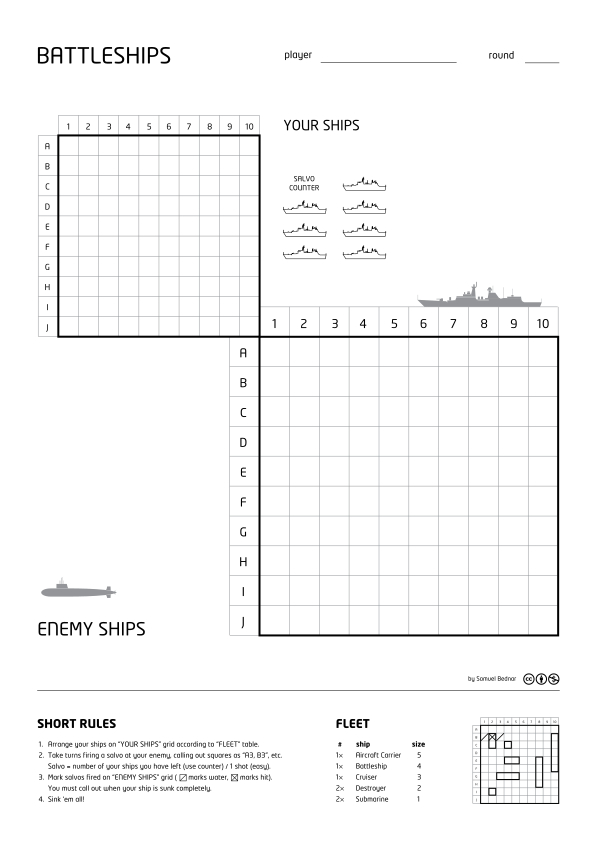
\includegraphics[width=.9\linewidth]{images/grillebn.jpg}
                \caption*{Grille de jeu}
                \label{fig:grillejeu}
            \end{subfigure}
            %\pause
            \begin{subfigure}{.56\textwidth}
                \centering
                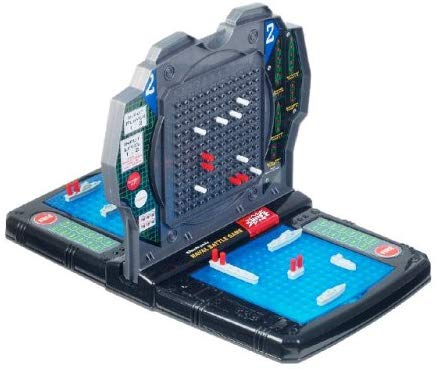
\includegraphics[width=.9\linewidth]{images/plateau.jpg}
                 \caption*{Plateau de jeu}
                \label{fig:plateaujeu}
            \end{subfigure}
        \end{figure}
    % Origine : jeu de société apparu après WW1 (A l'époque : "L'attaque")
    % Depuis 70's :  Plateau + succès commercial
	\end{frame}
	
	\begin{frame}{Contexte}
	    \begin{figure}
		    \begin{subfigure}{.50\textwidth}
    		    \centering
                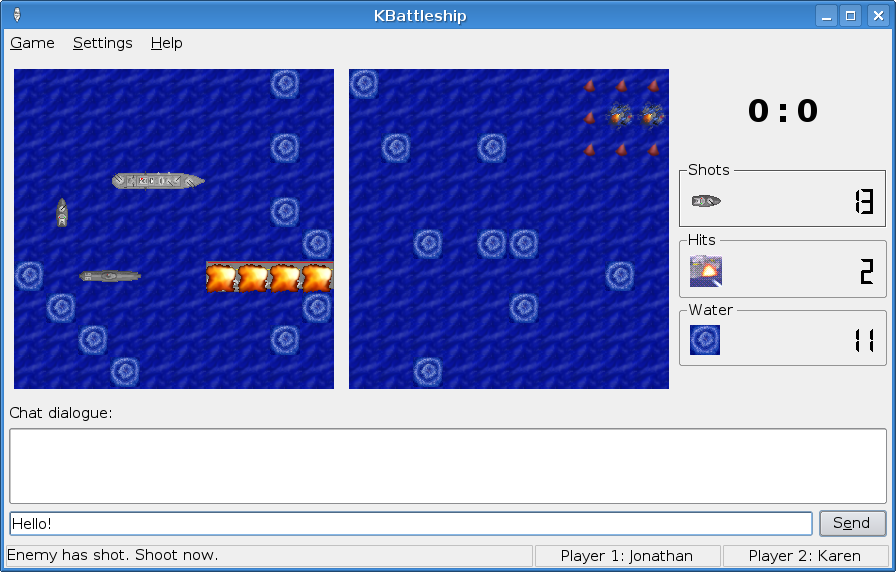
\includegraphics[width=.9\linewidth]{images/kbattleship.png}
                \caption*{Jeu en ligne : KBattleship}
                \label{fig:kbattleship}
            \end{subfigure}
            %\pause
            \begin{subfigure}{.48\textwidth}
                \centering
                
\includegraphics[width=.9\linewidth]{images/TODO.png} % TODO : ajouter capture
                 \caption*{Interface "Maison"}
                \label{fig:interfacemaison}
            \end{subfigure}
        \end{figure}
    % Aujourd'hui : jeux video
    % Droite : Notre interface -> module pygame
	\end{frame}
	
	\begin{frame}{Règles du jeu : notre variante}
	    \begin{block}{Plateau}
	        \begin{itemize}
	            \item Carré $10 \times 10$
	        \end{itemize}{}
	    \end{block}
	    %\pause
	    \begin{block}{Défenseur}
	        \begin{itemize}
	            \item 5 bateaux de longueur 2, 3, 3, 4, 5
	            \item Aucun contact (même en diagonale)
	        \end{itemize}{}
	    \end{block}
	    %\pause
	    \begin{block}{Attaquant}
	        \begin{itemize}
	            \item Tente de détruire la flotte adverse
	            \item Score : Nombre de coups nécessaire
	        \end{itemize}{}
	    \end{block}
	% Nous : schéma attaquant défenseur
	\end{frame}{}
	
	\begin{frame}{En pratique}
	    \begin{block}{Plateau : Interface Maison}
	        \begin{figure}
    		    \begin{subfigure}{.48\textwidth}
        		    \centering
        		    
\includegraphics[width=.9\linewidth]{images/TODO.png}
        		    % TODO : ajouter capture
                    \caption*{Défense}
                    \label{fig:plateaudefense}
                \end{subfigure}
                %\pause
                \begin{subfigure}{.48\textwidth}
                    \centering
                    
\includegraphics[width=.9\linewidth]{images/TODO.png} % TODO : ajouter capture
                     \caption*{Attaque}
                    \label{fig:plateauattaque}
                \end{subfigure}
            \end{figure}
	    \end{block}
	% Interface austère mais fonctionnelle
	\end{frame}{}
	
	\begin{frame}{En pratique}
	    \begin{block}{Défenseur}
	        \begin{itemize}
	            \item Aléatoire
	            \item Distribution uniforme sur l'ensemble des grilles valides
	        \end{itemize}{}
	    \end{block}
	    %\pause
	    \begin{block}{Attaquant}
	        \begin{itemize}
	            \item Intelligence artificielle
	        \end{itemize}{}
	    \end{block}
	    %\pause
	    \begin{block}{Définition : Intelligence artificielle}
	        \textit{}{Programme informatique capable de jouer correctement à la bataille navale.}
	    \end{block}
	% (Sauf mention du contraire)
    % Défenseur : pas notre but
    % "IA" -> vague, donc définition perso
	\end{frame}
	\section{Stratégies Probabiliste}

\subsection{Les différentes stratégies}
	
	\begin{frame}{Hasard}
		\begin{figure}
		    \centering
		    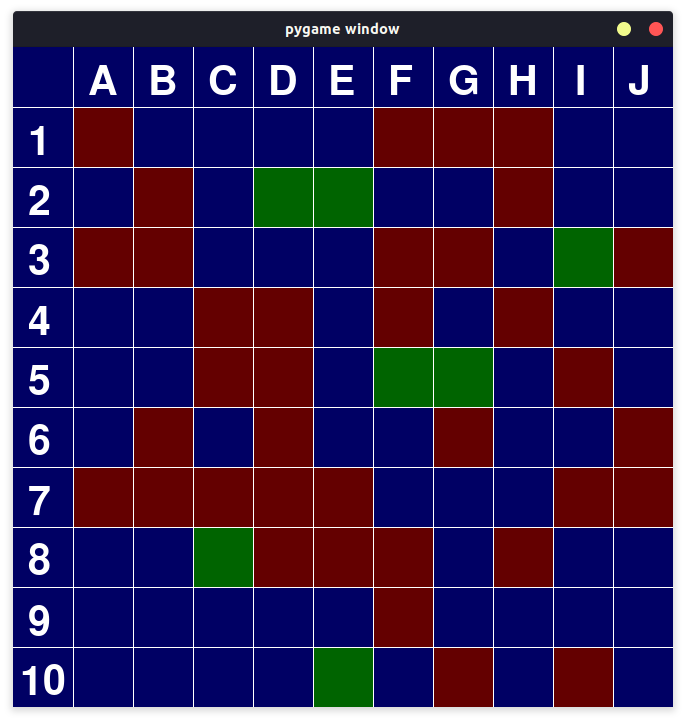
\includegraphics[width=.5\linewidth]{images/algoHasardMalin.png}
		    \caption*{Algorithme Hasard Malin}
		    \label{fig:algoHasardMalin}
		\end{figure}{}
	% Au hasard mais pas 2 fois sur la même case
	\end{frame}
	
	\begin{frame}{Chasse et Pêche}
	    \begin{figure}
		    \begin{subfigure}{.48\textwidth}
    		    \centering
    		    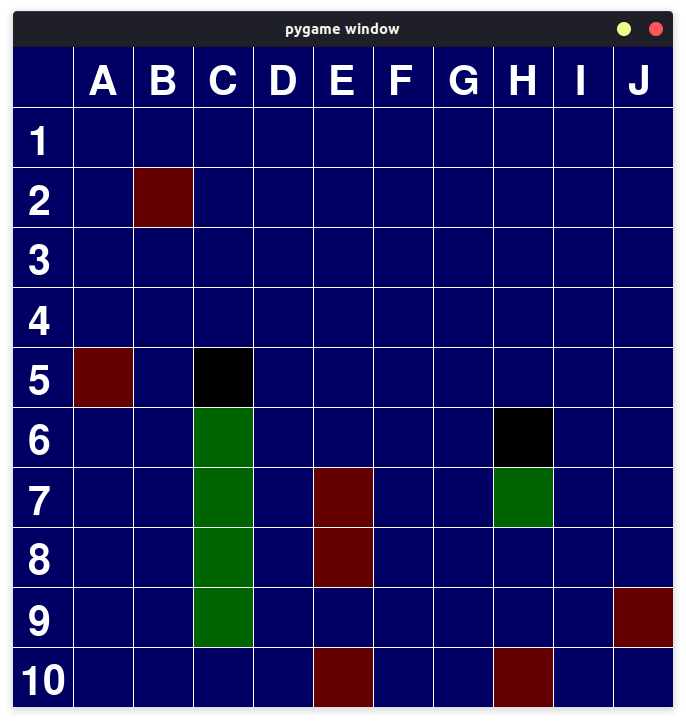
\includegraphics[width=.9\linewidth]{images/peche.png}
    		    % TODO : faire mieux pour chasse et peche
                \caption*{Chasse et Pêche Mode Pêche}
                \label{fig:CPpeche}
            \end{subfigure}
            %\pause
            \begin{subfigure}{.48\textwidth}
                \centering
                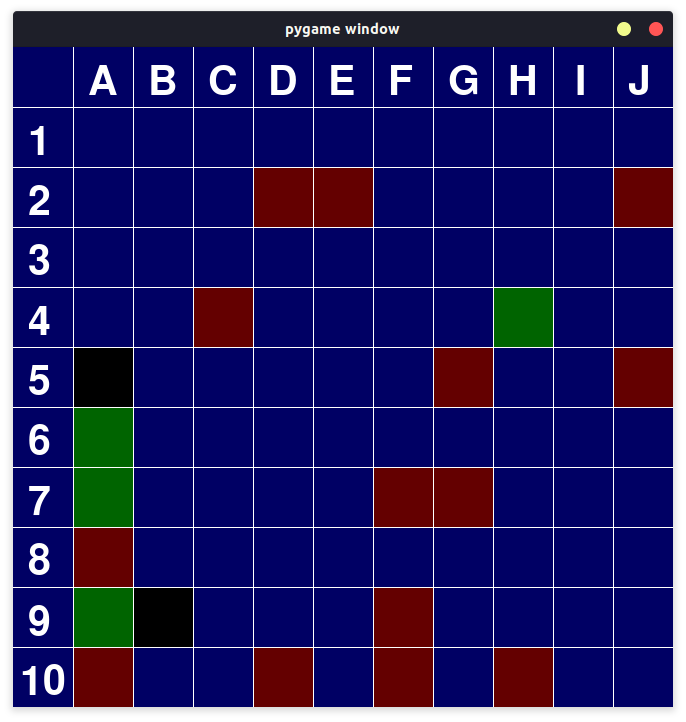
\includegraphics[width=.9\linewidth]{images/chasse.png}
                 \caption*{Chasse et Pêche Mode Chasse}
                \label{fig:CPchasse}
            \end{subfigure}
        \end{figure}
    % Explications
	\end{frame}{}
	
	\begin{frame}{Chasse Pêche Croix}
		\begin{figure}
		    \centering
		    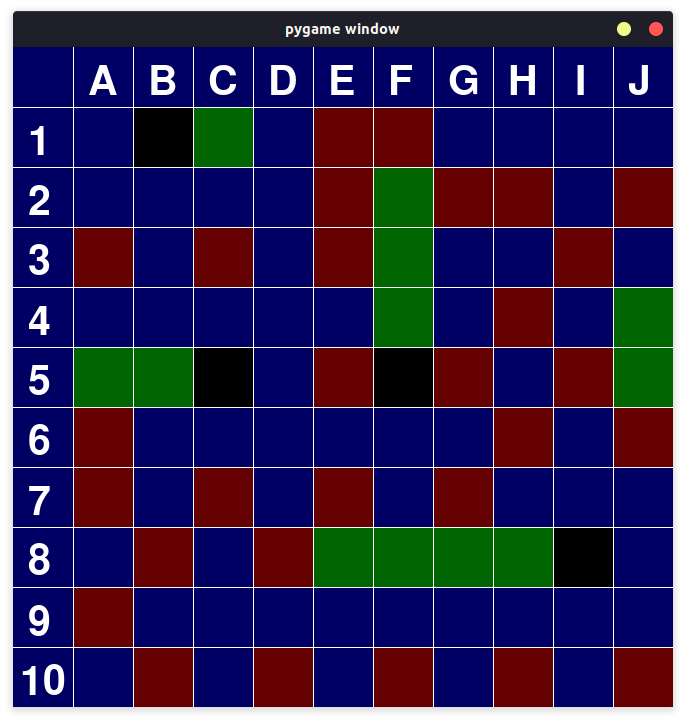
\includegraphics[width=.5\linewidth]{images/algoCPC.png}
		    \caption*{Algorithme Chasse Pêche Croix}
		    \label{fig:CPC}
		\end{figure}{}
	% Idem CP mais seumement une case sur deux car bateaux de taille 2 ou plus
	\end{frame}
	
	\begin{frame}{Chasse Pêche Proba}
	    \begin{figure}
		    \begin{subfigure}{.32\textwidth}
    		    \centering
    		    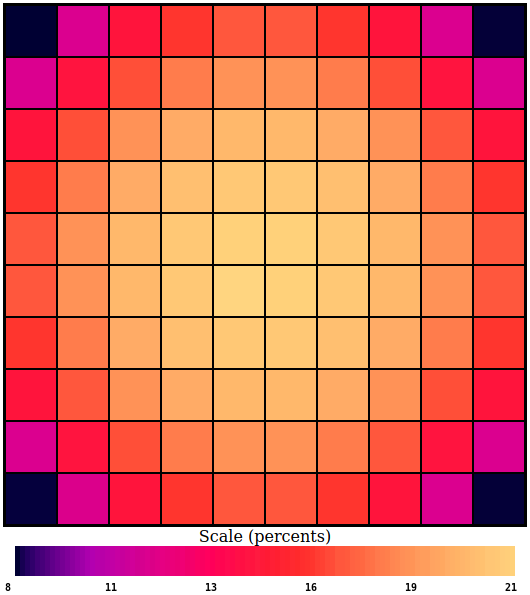
\includegraphics[width=.95\linewidth]{images/grille_initiale_proba.png}
                \caption*{Densité initiale}
                \label{fig:probaGrilleInit}
            \end{subfigure}
            %\pause
            \begin{subfigure}{.32\textwidth}
                \centering
                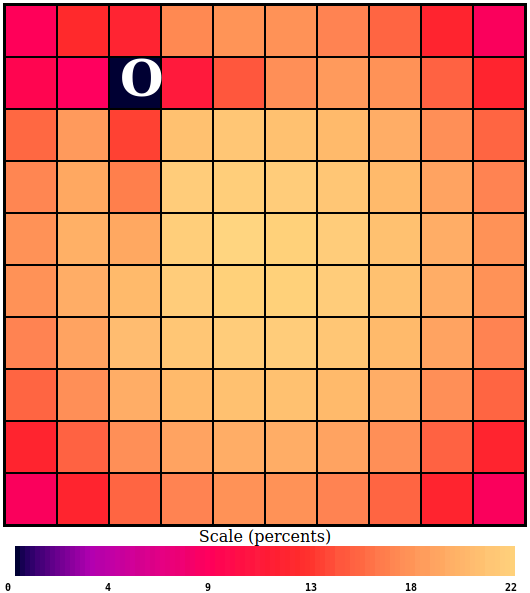
\includegraphics[width=.95\linewidth]{images/ploufC2.png}
                 \caption*{Plouf en C2}
                \label{fig:ploufC2}
            \end{subfigure}
            %\pause
            \begin{subfigure}{.32\textwidth}
                \centering
                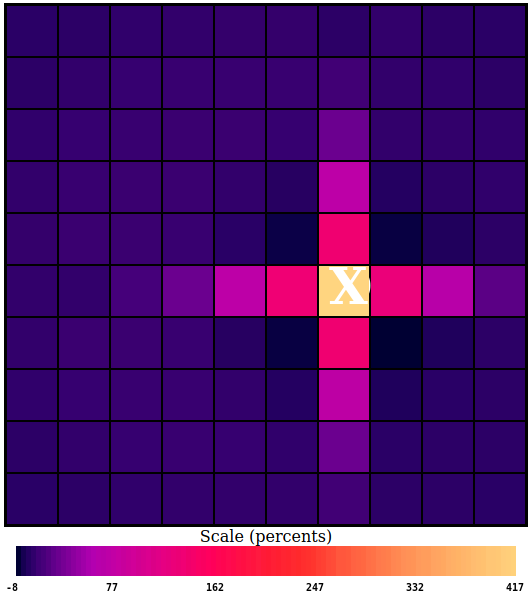
\includegraphics[width=.95\linewidth]{images/toucheG6.png}
                 \caption*{Touché en G6}
                \label{fig:toucheG6}
            \end{subfigure}
        \end{figure}
        \hfill Source : The Virtuosi
	\end{frame}{}
	
	\begin{frame}{Chasse Pêche Proba}
	    \begin{block}{Améliorations}
	        \begin{itemize}
	            \item Implémentation efficace : paradigme de programmation dynamique qui s'actualise en temps réel. Complexité en $\mathcal{O}(n\log{}n)$ %TODO : calculer la complexité
	            \item Prise en compte du nombre de bateaux et de leur taille
	            \item Mesure concrète de la qualité de l'algorithme
	        \end{itemize}
	    \end{block}
	\end{frame}{}
	
	\begin{frame}{Chasse Pêche Croix Proba}
	    \begin{block}{Algorithme Chasse Pêche Croix Proba}
	        \begin{itemize}
	            \item Algorithme perso
	            \item Mix entre CPC et CPP
	            \item Résultats médiocre 
	        \end{itemize}{}
	    \end{block}
	\end{frame}{}

\subsection{Résultats}
	
	\begin{frame}{Performances}
		\begin{figure}
		    \centering
		    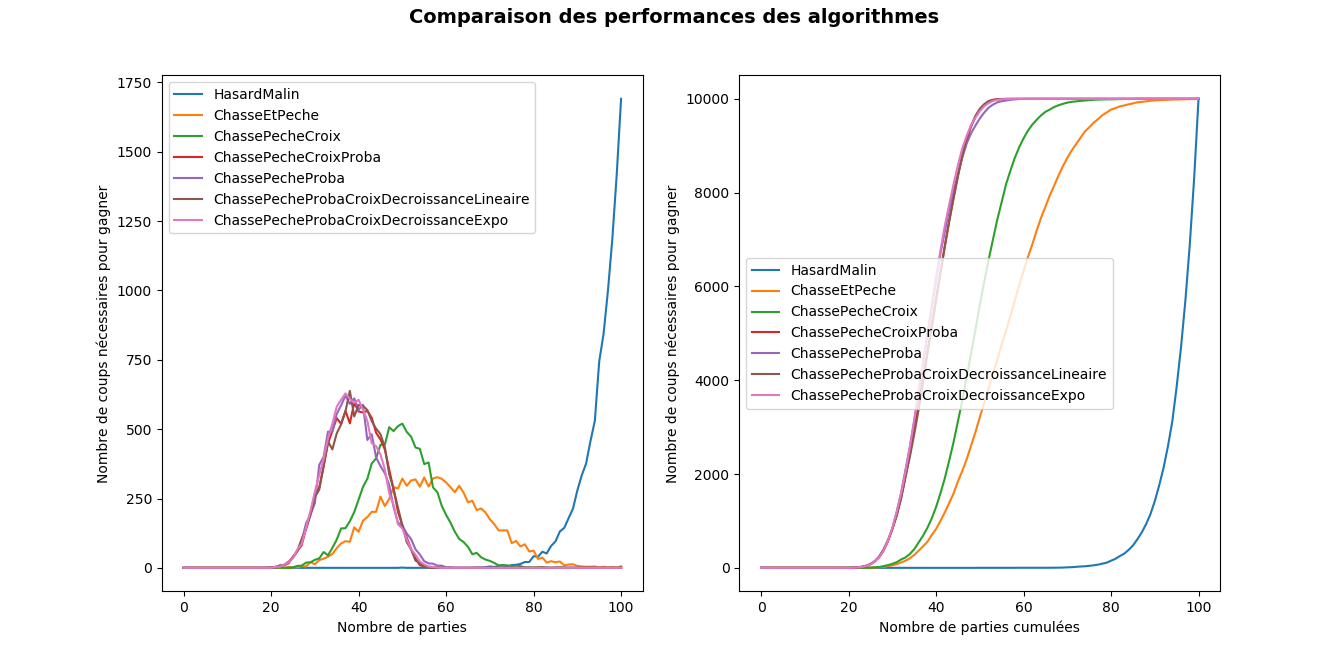
\includegraphics[width=.99\linewidth]{images/perfsstats.png}
		    \caption{Performances des différents algorithmes à stratégie probabiliste} % TODO : mettre les bons algos
		    \label{fig:perfsstats}
		\end{figure}{}
	\end{frame}
	\section{Apprentissage profond supervisé}

\subsection{L'IA "maison"}
	
	\begin{frame}3
		
	\end{frame}

\subsection{Tensoflow}
	
	\begin{frame}
		
	\end{frame}

\subsection{Résultats}
	
	\begin{frame}
		
	\end{frame}
	\section{Apprentissage profond par renforcement}
	\section{Conclusion}

\begin{frame}{Conclusion}
    \begin{block}{Objectifs du TIPE}
        \begin{itemize}
            \item[$\checkmark$] Implémenter un environnement et une interface permettant de jouer à la bataille navale
            \item[$\checkmark$] Concevoir et Implémenter plusieurs IA utilisant une stratégie probabiliste
            \item[$\checkmark$] Concevoir, implémenter depuis zéro et entraîner une IA utilisant l'apprentissage supervisé grâce à un
réseau de neurone
            \item[$\times$] Idem mais en utilisant une librairie, ici TensorFlow
            \item[$\times$] Concevoir, implémenter et entraîner une IA utilisant l'apprentissage par renforcement
            \item[$\checkmark$] Comparer les résultats et les performances temporelles des algorithmes
            %\item[$\checkmark$] Tirer une conclusion
        \end{itemize}{}
    \end{block}
\end{frame}{}

\begin{frame}{Conclusion}
    \begin{block}{Conclusion}
        Tous les outils présentés fonctionnent et permettent de créer des IA performantes, mais celle utilisant la \textbf{stratégie probabiliste} surpasse toutes les autres.
    \end{block}
\end{frame}

\begin{frame}{Travaux futurs}
    \begin{block}{}
        \begin{itemize}
            \item Concevoir une \textbf{IA de défense} qui place intelligemment les bateaux
            \item Concevoir une IA pouvant \textbf{jouer en 1V1} avec un avantage sur celle jouant dans sa bulle
            \item \textbf{Changer les règles} du jeu pour obtenir un jeu \textbf{plus fun} et dans lequel les IA de \textbf{Deep Learning seraient meilleures}
        \end{itemize}{}
    \end{block}
\end{frame}{}
	

\end{document}